%% ------------------------------------------------------------------------- %%
\chapter{Resultados}
\label{cap:resultados}

Neste capítulo apresentamos os resultados da avaliação do uso das redes convolucionais na recuperação de trecho de código-fonte. Utilizamos a nossa arquitetura proposta no Capítulo~\ref{cap:abordagem} e comparamos com outras duas arquiteturas: uma arquitetura de referência \textit{Embedding} e outra arquitetura que é o estado da arte em recuperação de trecho de código proposta por \citeonline{cambronero-deep-learning-code-search:2019}. Os resultados da arquitetura CNN foram promissores. A arquitetura apresentou um valor de métrica \acrfull{mrr} de $0,70$. Em $78\%$ das vezes, as respostas corretas apareceram entre as 3 primeiras posições, de um total de 50 possíveis respostas.

\section{Avaliação}
\label{sec:resultados-avaliacao}

Avaliamos a arquitetura CNN juntamente com outras duas arquiteturas, Embedding e \Gls{unif} na recuperação de trecho de código-fonte. Os resultados foram coletados a partir da amostra \emph{EVAL} e o valor final MRR é a média obtida após 20 iterações. Conforme a Tabela~\ref{table:resultados}, as arquiteturas CNNs compartilhadas com 4000 filtros convolucionais (linhas D3 e F3) obtiveram o melhor resultado. A arquitetura CNN obteve uma média MRR 5\% superior ao melhor resultado obtido pela arquitetura Unif (linha B1), atual estado da arte. Um resultado 11\% superior foi obtido em relação à arquitetura de referência Embedding (linha A1). 

\begin{table}[H]
\centering
\caption[Resultado do modelo CNN em comparação com as outras arquiteturas \Gls{unif} e Embedding.]{Resultado do modelo CNN em comparação com as outras arquiteturas \Gls{unif} e Embedding. MRR refere-se a média do resultado do Mean Reciprocal Rank (equação~\ref{eq:mrr}) na amostra EVAL. TOP1 refere-se a frequência da ocorrência da resposta anotada como correta na primeira posição em comparação com outros 49 distratores. Nas linhas A1 e B1, \emph{m} refere-se ao hiper-parâmetro margem utilizada na função de perda \emph{hinge}. F indica a quantidade de filtros convolucionais utilizados durante o treinamento das redes convolucionais. NL é o acrônimo de normalização em lote. As arquiteturas CNN utilizaram margem $m = 0.05$ e o tamanho da janela do filtro (kernel) $k = 2$. }
\begin{tabular}{ p{1cm} p{6cm} P{4cm} P{4cm} }
 \hline
    & & \multicolumn{2}{c}{\textbf{Resultados}}\\
 \hline
 & \textbf{Modelos} & \textbf{MRR} & \textbf{TOP1}\\
 \hline
 A1 & Embedding (m = $0.1$) & $0.637$& $0.493 \pm 0.009$\\
 
 \hline
 
 B1 & Unif (m = $0.2$) & $0.675 \pm 0.006$ & $0.539 \pm 0.009$\\
 
 \hline
 
 C1 & CNN / F = 1000 & $0.669 \pm 0.006$ & $0.527 \pm 0.012$\\
 
 C2 & CNN / F = 2000 & $0.673 \pm 0.007$ & $0.531 \pm 0.012$\\
 
 C3 & CNN / F = 4000 & $0.687 \pm 0.006$ & $0.553 \pm 0.011$\\
 
 \hline
 
 D1 & CNN Compartilhado / F = 1000 & $0.678 \pm 0.007$ & $0.548 \pm 0.012$\\
 
 D2 & CNN Compartilhado / F = 2000 & $0.694 \pm 0.008$ & $0.565 \pm 0.012$\\
 
 D3 & CNN Compartilhado / F = 4000 & $0.700 \pm 0.004$ & $0.569 \pm 0.009$\\
 
 \hline
 
 E1 & CNN com NL / F = 1000 & $0.682 \pm 0.007$ & $0.543 \pm 0.012$\\
 
 E2 & CNN com NL / F = 2000 & $0.689 \pm 0.006$ & $0.553 \pm 0.011$\\
 
 E3 & CNN com NL / F = 4000 & $0.688 \pm 0.006$ & $0.553 \pm 0.011$\\
 
 \hline
 
 F1 & CNN Compartilhado com NL / F = 1000 & $0.690 \pm 0.008$ & $0.553 \pm 0.015$\\
 
 F2 & CNN Compartilhado com NL / F = 2000 & $0.700 \pm 0.007$ & $0.573 \pm 0.012$\\
 
 F3 & CNN Compartilhado com NL / F = 4000 & $0.701 \pm 0.008$ & $0.577 \pm 0.015$\\
 
\hline
\end{tabular}
\source{Tabela do artigo \citeonline{martins2020concra}.}
\label{table:resultados}
\end{table}

Conforme os resultados da Tabela~\ref{table:resultados}, o aumento da quantidade de filtros convolucionais resultou em uma melhora no desempenho do modelo (linhas D3 e F3). O aumento da quantidade de filtros aumenta o grau de liberdade do modelo, resultando em um aumento da capacidade de aprendizagem da rede convolucional (ver Equação~\ref{eq:feature-map}). As redes convolucionais que compartilharam os parâmetros (linhas D e F) obtiveram um desempenho superior aos modelos que utilizaram parâmetros independentes (linhas C e E). Para \citeonline{wen-joint-modeling-question-answer-2019}, as redes convolucionais que aprendem as representações de forma independente e postergam a interação entre elas para a última camada (cálculo da similaridade), exploram de forma ineficiente a correlação semântica entre as respectivas representações dos pares de questões e respostas. No nosso caso, verificamos que ao treinar por mais épocas, não houve melhora significativa no desempenho, salientando a dificuldade das redes convolucionais em encontrar uma correlação semântica entre os pares de questões e respostas.

Durante o treinamento, para evitar o \textit{overfitting} dos modelos, adotamos a técnica de normalização em lote, que além de melhorar o desempenho, a velocidade e a estabilidade das redes neurais, mitiga o \textit{overfitting}, reduzindo a necessidade do uso de outra técnica de regularização como o \textit{dropout} \cite{sergey-batch-normalization-2015}. No nosso caso, verificamos a melhora no desempenho e robustez das redes convolucionais (ver linhas E e F da Tabela~\ref{table:resultados} e ver Apêndice~\ref{ape:ajuste-hiper-parametros-cnn}). No caso da arquitetura Unif, optamos por manter a arquitetura padrão proposta por \citeonline{cambronero-deep-learning-code-search:2019}. Para a arquitetura \textit{Embedding}, não houve a necessidade de regularização.

A Figura~\ref{fig:histogram-mrr} exibe as posições da primeira ocorrência do trecho de código-fonte encontradas durante a avaliação dos modelos. Tanto o CNN quanto a arquitetura Unif conseguiram classificar os trechos de código-fonte entre as três primeiras posições em 75\% dos casos. A nossa arquitetura proposta obteve uma precisão TOP-1 de aproximadamente 60\%, i.e., em aproximadamente 60\% das vezes, o trecho de código-fonte relevante foi observada na primeira posição. A arquitetura Unif e Embedding obtiveram uma precisão TOP-1 de pouco mais de 50\%. 


\begin{figure}[h]
    \centering
    \caption[Figura das primeiras posições observadas para o trecho de código-fonte anotado como correto.]{Figura das primeiras posições observadas para o trecho de código-fonte anotado como correto. As legendas \emph{shared-cnn-with-bn}, \emph{unif} e \emph{embedding} referem-se as linhas F3, A1 e B1 da Tabela~\ref{table:resultados} respectivamente. }
    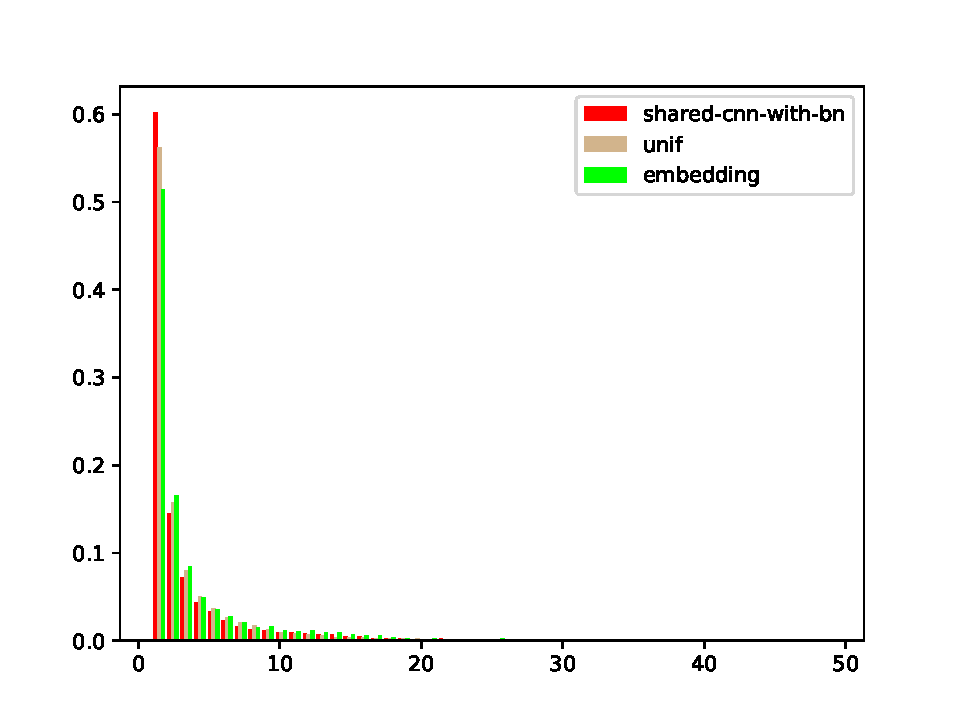
\includegraphics[width=1\textwidth]{figuras/cap-resultados/histogram.pdf}
    \source{Figura do artigo \citeonline{martins2020concra}.}
    \label{fig:histogram-mrr}
\end{figure}

\section{Ameaças à validade}

Conforme citado anteriormente, \citeonline{yao-2018} anotaram o conjunto de dados utilizando um framework proposto em seu artigo. Para anotá-los, os autores treinaram uma rede neural no conjunto de dados anotado manualmente. Em nosso trabalho, fizemos o caminho inverso. Treinamos os nossos modelos nos dados anotados automaticamente e avaliamos no conjunto anotado manualmente. Para diminuir o viés, adotamos o procedimento proposto por \citeonline{iyer-etal-2016-summarizing} descrito na Seções~\ref{sec:treinamento} e \ref{sec:avaliacao}.
Além disso, utlizamos apenas a linguagem Python para os experimentos e coleta dos resultados. As suas principais características como sintaxe concisa e clara podem ter influenciados os resultados obtidos pela nossa arquitetura. 

\section{Considerações}
\label{sec:consideracoes-resultados}

Os resultados são prominentes e a arquitetura proposta obteve um bom desempenho na recuperação de trecho de código-fonte. Algumas considerações a respeito do experimento e dos resultados das redes convolucionais:

\begin{itemize}
    \item Não houve a necessidade de um tratamento especial para os trechos de código em Python, devido às suas características, como sintaxe mais concisa, clara e muito menos verbosa quando comparada a outras linguagens \cite{theodora-introductory-programming-python-2015}, facilitando a extração das palavras durante o pré-processamento. 
    
    \item Em nosso estudo, utilizamos \gls{word2vec} para mapear as palavras para vetores contínuos, porém recentes avanços em NLP apresentaram outras soluções como os \textit{transformers} \cite{attention-is-all-you-need-2017}. Trabalhos futuros podem investigar como esses recentes avanços podem auxiliar na recuperação de trecho de código-fonte.
    
    \item No nosso trabalho, utilizamos questões em inglês extraídas do Stack Overflow. Isso facilitou bastante o treinamento das redes neurais, pois permitiu a criação de um vocabulário único formado pelo conjunto de palavras presentes nas questões e nos trechos de código-fonte. Trabalhos futuros podem explorar as questões e as respostas em português do Stack Overflow. Neste caso, acreditamos que será necessário a criação de vocabulários distintos, um para as questões e outro para os trechos de código-fonte, acarretando um tempo maior para o treinamento. Mais informações sobre os vocabulários estão presentes na Seção~\ref{sec:abordagem-representacao-token}.
    
    \item Segundo \citeonline{Goodfellow-et-al-2016}, as redes convolucionais não conseguem correlacionar palavras muito distantes em um sentença. No nosso caso, isto não foi um problema, pois conforme apontado na Tabela~\ref{table:statistical-descriptive-of-pythons-sample}, 75\% das questões das nossas amostras tem 11 palavras no máximo, enquanto 75\% dos trechos de código tem no máximo 55 palavras.
    
    \item Adotamos a métrica MRR que indica o quanto um modelo está conseguindo classificar a informação relevante entre as primeiras posições. O CNN (linha F3 da Tabela~\ref{table:resultados}) conseguiu classificar o trecho anotado como correto entre as 3 primeiras posições em 78\% dos casos. Porém, somente a métrica MRR não é suficiente, é necessário investigar e analisar estes resultados de forma qualitativa. Um estudo futuro pode verificar e validar estes resultados com usuários finais, por exemplo. 
\end{itemize}


